\documentclass[12pt,reqno]{amsart}
\usepackage[letterpaper,margin=1in,footskip=1in]{geometry}
\usepackage{microtype}
\usepackage[only,llbracket,rrbracket]{stmaryrd}
\usepackage{enumitem}
\usepackage{amsmath}
\usepackage{amssymb}
\usepackage{mathtools}
\usepackage{tikz-cd}
\usepackage{mathrsfs}
\usepackage{verbatim}
\usepackage{subfig}
\usepackage{comment}
\usepackage[justification=centering]{caption}
\usepackage[noadjust]{cite}
\renewcommand{\citepunct}{;\penalty\citemidpenalty\ }
\usepackage{combelow}
\linespread{1.05}
\PassOptionsToPackage{pdfusetitle,pagebackref,colorlinks,bookmarksdepth=3}{hyperref}
\usepackage{bookmark}
\hypersetup{citecolor=[HTML]{2E7E2A},linkcolor=[HTML]{000000},urlcolor=[HTML]{8A0087}}
\newtheorem{theorem}{Theorem}[section]
\newtheorem{lemma}[theorem]{Lemma}
\newtheorem{cor}[theorem]{Corollary}
\newtheorem{proposition}[theorem]{Proposition}
\newtheorem{corollary}[theorem]{Corollary}
\newtheorem{question}[theorem]{Question}
\newtheorem{innercustomthm}{Theorem}
\newenvironment{customthm}[1]
  {\renewcommand\theinnercustomthm{#1}\innercustomthm}
  {\endinnercustomthm}

\newtheorem{alphthm}{Theorem}
\renewcommand{\thealphthm}{\Alph{alphthm}}

\theoremstyle{definition}
\newtheorem{definition}[theorem]{Definition}
\newtheorem{example}[theorem]{Example}
\newtheorem{setup}[theorem]{Setup}
\newtheorem{construction}[theorem]{Construction}

\theoremstyle{remark}
\newtheorem{remark}[theorem]{Remark}
\newtheorem{conjecture}[theorem]{Conjecture}

\newtheoremstyle{citedrem}{.5\baselineskip\@plus.2\baselineskip\@minus.2\baselineskip}{.5\baselineskip\@plus.2\baselineskip\@minus.2\baselineskip}{}{}{\itshape}{\itshape .}{5pt plus 1pt minus 1pt}{\thmname{#1}\thmnumber{ \normalfont#2}\thmnote{ \normalfont#3}}
\theoremstyle{citedrem}
\newtheorem{citedrem}[theorem]{Remark}

\newtheoremstyle{cited}{.5\baselineskip\@plus.2\baselineskip\@minus.2\baselineskip}{.5\baselineskip\@plus.2\baselineskip\@minus.2\baselineskip}{\itshape}{}{\bfseries}{\bfseries .}{5pt plus 1pt minus 1pt}{\thmname{#1}\thmnumber{ #2}\thmnote{ \normalfont#3}}
\theoremstyle{cited}
\newtheorem{citedthm}[theorem]{Theorem}
\newtheorem{citedlem}[theorem]{Lemma}
\newtheorem{citedprop}[theorem]{Proposition}
\newtheorem{citedques}[theorem]{Question}

\newtheoremstyle{citeddef}{.5\baselineskip\@plus.2\baselineskip\@minus.2\baselineskip}{.5\baselineskip\@plus.2\baselineskip\@minus.2\baselineskip}{}{}{\bfseries}{\bfseries .}{5pt plus 1pt minus 1pt}{\thmname{#1}\thmnumber{ #2}\thmnote{ \normalfont#3}}
\theoremstyle{citeddef}
\newtheorem{citeddef}[theorem]{Definition}

\newtheoremstyle{step}{.25\baselineskip\@plus.1\baselineskip\@minus.1\baselineskip}{.25\baselineskip\@plus.1\baselineskip\@minus.1\baselineskip}{\itshape}{}{\bfseries}{\bfseries .}{5pt plus 1pt minus 1pt}{\thmname{#1}\thmnumber{ #2}\thmnote{ \normalfont(#3)}}
\theoremstyle{step}
\newtheorem{step}{Step}[theorem]
\renewcommand{\thestep}{\arabic{step}}
\newtheorem{claim}{Claim}[theorem]
\newtheorem{subclaim}{Subclaim}[claim]

\DeclareMathOperator{\Min}{Min}
\DeclareMathOperator{\Spec}{Spec}
\DeclareMathOperator{\height}{ht}

\usepackage{minitoc}
\usepackage{nameref} % Note: Do not load it before minitoc ! 

\newcommand{\Z}{\mathbb{Z}}
\newcommand{\Q}{\mathbb{Q}}
\newcommand{\N}{\mathbb{N}}
\newcommand{\F}{\mathbb{F}}
\newcommand{\R}{\mathbb{R}}
\newcommand{\C}{\mathbb{C}}
\newcommand{\A}{\mathbb{A}}
\newcommand{\ZZ}{\mathbf{Z}}
\newcommand{\bP}{\mathbf{P}}
\newcommand{\fN}{\mathfrak{N}}
\newcommand{\fm}{\mathfrak{m}}
\newcommand{\fp}{\mathfrak{p}}
\newcommand{\fq}{\mathfrak{q}}
\newcommand{\fa}{\mathfrak{a}}
\newcommand{\fb}{\mathfrak{b}}
\newcommand{\gr}{\mathrm{gr}}
\newcommand{\red}{\mathrm{red}}
\newcommand{\spec}{\mathrm{Spec}}
\newcommand{\an}{\mathrm{an}}
\newcommand{\na}{\mathrm{na}}
\newcommand{\val}{\mathrm{Val}}
\renewcommand{\div}{\mathrm{div}}
\newcommand{\fvol}{\mathrm{Fvol}}
\newcommand{\vol}{\mathrm{vol}}
\newcommand{\nvol}{\widehat{\mathrm{vol}}}
\newcommand{\fpt}{\mathrm{fpt}}
\newcommand{\lct}{\mathrm{lct}}
\newcommand{\QM}{\mathrm{QM}}
\newcommand{\hooklongrightarrow}{\lhook\joinrel\longrightarrow}
\newcommand{\ord}{\mathrm{ord}}
\newcommand{\FS}{\mathrm{FS}}
\newcommand{\MA}{\mathrm{MA}}
\newcommand{\triv}{\mathrm{triv}}
\usepackage{contour}
\usepackage[normalem]{ulem}
\renewcommand{\ULdepth}{1.8pt}
\contourlength{0.8pt}
\newcommand{\myuline}[1]{%
  \uline{\phantom{#1}}%
  \llap{\contour{white}{#1}}%
}

\providecommand\given{}
\newcommand\SetSymbol[1][]{\nonscript\:#1\vert\allowbreak\nonscript\:\mathopen{}}
\DeclarePairedDelimiterX\Set[1]\{\}{\renewcommand\given{\SetSymbol[\delimsize]}#1}

\tikzcdset{scale cd/.style={every label/.append style={scale=#1},cells={nodes={scale=#1}}}}
\newcommand{\ben}[1]{{\textcolor{blue}{B: #1}}}
\newcommand{\ying}[1]{{\textcolor{purple}{Y: #1}}}

\begin{document}
\title{Summary of Chambert-Loir--Ducros}
%\thanks{}

\author[Ying Wang]{Ying Wang}
\begin{abstract}This is my summary of the French monograph by Chambert-Loir--Ducros, which develops a local theory of pluripotential functions on analytic spaces. All errors are mine and corrections are always welcome. 
\end{abstract}
%\address{Department of Mathematics\\University of Michigan\\Ann Arbor, MI 48109-1043\\USA}

%\subjclass[2020]{Primary }

%\keywords{}

%\makeatletter
%\hypersetup{
%  pdfauthor={}
%}
%\makeatother


\maketitle

\section*{Part 1: Tropical Geometry}

\subsection*{Chapter 1: Superforms on Real Vector Spaces}

\subsubsection*{1.1-1.2: Superforms.}
Let $V$ be a real vector space of dimension $n < \infty$. For any $0 \leq p, q \leq n$, the space of $(p,q)$-(super)forms on $V$ is denoted by $A^{p,q}$. These are forms with real coefficients, and have various positivity notions.

\begin{remark}
    We will often omit the prefix super. 
\end{remark}

\subsubsection*{1.3-4: Superforms with coefficients.}
For any $U \subseteq V$ open, the differential superforms of type $(p,q)$ is $\mathscr{A}^{p,q}_V(U) = C^\infty(U) \otimes_{\mathbf{R}} A^{p,q}(V).$ They form a graded algebra and has a natural ($\pm 1$)-involution $J$, giving rise the definition of symmetric forms. There are two differentials $d', d''$ on these differential superforms. Under the tropicalizatio map $(\mathbf{C}^\ast)^n \to V$ by $z_i \mapsto \log|z_i| = x_i$, the form $d'x_i$ correspond to $d\log|z_i|$ and $d''x_i$ correspond to $d\mathrm{arg}(z_i)$. 

One can replace $C^\infty$ by other sheaves on $V$ and obtain superforms with different coefficients. 

\subsubsection*{1.5: Integrating a $(p,n)$-form on $p$-dimensional subspace.} Given an abstract vector space $V$ of dimension $n$, the integration of a $(p,n)$-form with Borel coefficients (on an $p$-dimensional subspace of $V$) strongly depend on the choice of identification between $V$ and $\mathbf{R}^{\dim n}$. The fix to this is to specify a volume vector $\mu = (\lambda, O) \in |\Lambda^n V| \coloneqq \Lambda^n V \times^{\{\pm 1\}} \mathrm{Or}(V)$. This is equivalent to choosing an oriented coordinate system on $V$. Using a vector volume, one can constract the $d''$-part of an $(n,n)$-form $\omega$ to get a measure, written as $\langle \omega, \mu \rangle$. A vector volume also canonically induces vector volumes on boundaries of half-spaces, and as such we have Stokes' and Green's formulae. 


\subsubsection*{1.6: Supercurrents.} The space of smooth, compactly supported $(p,q)$-forms on $V$ has a locally convex topology. The topological dual is the supercurrents of bimension $(p,q)$. Supercurrents have operators $d',d''$, positivity, Poincar\'{e} lemma for $(1,1)$-currents, and include superforms as a subspace. Moreover, if $f$ is continuous on $V$, then $d'd''f$ is positive iff $f$ is convex. By convolution, supercurrents can be computed as locally uniform limits of superforms. For any $f$ convex, by approximation the $(n,n)$-supercurrent $(d'd''f)^n$ is a positive measure on $V$, and is the same as the real MA measure $\MA(f)$. This can be inductively defined as $d'd''(f (d' d''f)^{k-1}).$ If $\phi$ is $C^2$, then \[\MA(\phi) = n!\det(\frac{\partial^2 \phi}{\partial x_i \partial x_j}) d'x_1 d''x_1 \cdots d'x_n \wedge d''x_n.\]

\begin{remark}
    $(1,1)$-supercurrents are closely related to tropical geometry. For example, for a tropical polynomial $g = \max\{$affine functionals $f_i \}$, we have $d'd''g = \sum_k [V(f_i)] \wedge d''v_i$, where $v_i$ is a weighted normal to $V(f_i)$. It is a closed positive current with $(n-1)$-dimensional support iff the balancing condition for $\mathrm{trop}(g)$ holds. See \cite{Lag12} \S 5 for details. 
\end{remark}

\subsubsection*{1.7: Calculations of MA operator.} A collection of affine functionals $\{f_i\}_1^m$ on $V$ is very separating if the induced map $(f_i - f_j)_i \colon V \to \mathbf{R}^m$ is injective for some (and hence any) fixed $1 \leq j \leq m$. The following proposition shows that the MA operator is related to intersection theory. 

\begin{proposition}
    Let $V$ be a real vector space of dimension $n$ ,and $(f_1, \cdots, f_m)$ be a family of affine functions on $V$. Let $g = \max_j f_j$. For any $x \in V$, let $I_x \coloneqq \{i \in [m] \colon f_i = g\}$. Let $S$ be the set of $x \in X$ such that $I_x$ is very separating. Then $S$ is finite, and we can calculate $(d'd''g)^n = \sum_{x \in S} \lambda_x \delta_x$ where $\lambda_x > 0$ for any $x \in S$. 
\end{proposition}

\subsubsection*{1.8: Cells and polyhedrons.}
Let $V, W$ be affine spaces, and $P \subseteq V$ a polyhedron. We say a map $f\colon P \to W$ is piecewise-linear (PL) if there is a locally finite family of cells $\{C_i\}$ in $V$ whose union is $P$, such that for all $i$, the restriction $f|_{C_i}$ can be realized as the restriction of an affine map $V \to W$. Any subset $X \subseteq V$ is called a PL subspace if it is $G$-covered by the cells (usually defined) it contains. Any PL subspaces are locally closed, and the closed PL subspaces are polyhedra. All open subsets are PL subspaces. 

We define $G$-covering of subsets of a topological space, which are coverings by PL subspaces, and then define the tangent space to a point in a PL subspace of an affine space. This leads to a G-topology on $V$, which is denoted $V_G = (\mathrm{Dom}(V), \{G$-coverings$\})$, where $\mathrm{Dom}(V)$ consists of all PL subspaces of $V$. In particular, open subsets are PL and open coverings are G-coverings.

\subsubsection*{1.9: Differential forms on a PL subspace.} Let $V$ be an affine space, $U$ any open, $C$ any cell in $U$, and $P$ any PL subsapce in $U$. For any form $\omega \in \mathcal{F}^{p,q}(U)$, we define the meaning of $\omega|_C = 0$, and thereby $\omega|_P = 0$.

The zeroness is $G$-local under any PL coverings. There is a sub-sheaf $\mathcal{N}_P^{p,q}$ of zero forms on $P$. Let $j \colon P \hookrightarrow V$ be the embedding, and we define $\mathcal{F}_P^{p,q} \coloneq j^{-1}(\mathcal{F}^{p,q}_V / \mathcal{F}^{p,q}_V \cap \mathcal{N}_P^{p,q}))$. We can analogously define the sheaves in the G-topology. 

\begin{example}
    Let $P = \{y=0\} \subseteq \mathbf{R}^2$. Then $\omega = dy$ has a paradoxical property: $\omega(p,0) = dy$ on $\mathbf{R}^2$ for any $(p,0) \in P$, but $\omega|_P = 0$ as a form on $P$. The definition above captures the latter phenomenon in the sense that $\omega \in \mathcal{N}_P^{1,0}$. 
\end{example}

\begin{lemma}
    If $P = C$ is a cell, then for any $U \subseteq \mathbf{R}^n$ open, we have $\mathcal{F}^{p,q}_P = \mathcal{F}^{0,0}_P \otimes_{\mathbf{R}} \mathcal{A}^{p,q}(\langle C\rangle)$, where $\langle C \rangle$ is the affine space generated by $C$. 
\end{lemma}

\begin{example}
    This fails for general PL subspaces $P$. For example, tale $P$ to be $\{x = 0\} \cup \{y = 0\} \subseteq \mathbf{R}^2$. Then $d'x \wedge d''y = 0$ in $\mathcal{A}_P^{1,1}(P)$ but is not zero in $\mathcal{A}^{1,1}(\mathbf{R}^2)$.
\end{example}

\begin{remark}
    The sheaf $\mathcal{F}^{p,q}_{V_G}$ is G-separated. 
\end{remark}

\subsubsection*{1.10: Positive $G$-forms on PL subspaces.}

Let $C$ be a cell. For any $\omega \in \mathcal{F}^{p,q}_C(C)$, its positivity is defined by evaluation at any point $x \in C$. By covering PL subspaces $P$ by cells, one can define positivity of forms on $P$ as well. We define a sheaf $\mathrm{CConv}_P$ to be the smallest subsheaf of the sheaf of continuous functions on $P$ that satisfy the following two properties: 
\begin{itemize}
    \item it contains all the smooth functions $u$ on an open subset of $P$ with $d' d'' u$ positive, 
    \item it is stable under uniform limits. 
\end{itemize}
If $P$ is a cell, then a function is in this sheaf iff it is convex in the usual sense. 

\subsection*{Chapter 2: PL Spaces}
\subsubsection*{2.1: Various definitions.}
Let $X$ be a separated topological space. A PL chart on $X$ is a locally closed subset $P$ on $X$ with a continuous function $\phi\colon P \to V$, where $V$ is real affine space, such that $\phi$ is a homeomorphism onto a PL subspace of $V$. If $\phi(P)$ is a cell, this is called a cellular chart. Notions of equivalent charts are introduced, and $X$ is a PL space if it has a maximal class of PL charts. 

Let $f\colon X \to Y$ be a map of PL spaces. We say $f$ is a piecewise immersion if there is a $G$-covering $\{P_i\}$ of PL subspaces of $X$ such that $f|_{P_i}$ is a homeomorphism onto its image, and the image is PL in $Y$.

\subsubsection*{2.2: Cellular decomposition.}

Let $X$ be a PL space and $C \subseteq X$ a subset. Two cellular charts $(C, f), (C, g)$ are equivalent if $g \circ f^{-1} \colon f(C) \to g(C)$ is the restriction of an affine map. Such an equivalent class $(C,f)$ is called a strong cell. See definition 2.2.4 for the axioms of a cellular decomposition of $X$. Now we have two types of structures on a PL space $X$, namely atlases and cellular decompositions, and the there is a notion of adapation (Def 2.2.11). If the atlas is locally finite and takes value in cells, then adapted cellular decomposition always exists (Proposition 2.2.15). 

\subsubsection*{2.3: Relative cellular decomposition.} Given a map $f \colon X \to Y$ a PL map between PL spaces with respective cellular decomposition $(X, \mathcal{C})$ and $(Y, \mathcal{D})$, we can discuss how $f$ interacts with the cells. Definition 2.3.1 defines what it means for $(\mathcal{C}, \mathcal{D})$ to be adapted to $f$, and this section proves various existence results for cellular decompositions adapted to a map. 

\subsection*{Chapter 3: $G$-Tropical Spaces}

\subsubsection*{3.1: $G$-tropical spaces.} If a separated topological space $X$ has a $G$-topology, where the domains are certain locally closed subsets of $X$ satisfying the axioms, we can define a $G$-sheaf $\mathrm{PL}_X$ of PL functions axiomatically. To get a feeling of the axioms, we need that for any compact $W \subseteq X$, a PL map $f$ (i.e., each component is a PL function) should map $W$ to a PL subspace of $\mathbf{R}^m$; conversely, inverse image $f^{-1}(P)$ is a domain on $X$ for any PL subspace $P$ in $V$. A $G$-tropical chart on $X$ is a triple $(V, f, P)$, where $V$ is a domain on $X$, $f\colon V \to E$ is a PL map to some affine space $E$, and $P$ is a PL subspace of $E$ containing $f(V)$. (Note that since $V$ is only locally closed, $f(V)$ may not be a PL subspace.) In reality, we can often assume $P = E$ and omit it. If $x \in V$, then the tropical dimension of $f$ at $x$ is defined to be \[\mathrm{dim}_{\mathrm{trop},x}(f)\coloneqq \inf_{x \in W \subseteq V} \dim (f(W))\] where $W$ is any compact subset of $V$ that is a neighborhood of $x$. Using this, the tropical dimension of $x$ is \[\dim_{\mathrm{trop}}(x) \coloneqq \sup_{(V,f)} \dim_{\mathrm{trop},x}(f),\] and the tropical dimension of $X$ is \[\dim_{\mathrm{trop}}(X) \coloneqq \sup_{x \in X} \dim_{\mathrm{trop}}(x).\] For any $n \in \mathbf{N}$, we define \[X^{(n)} = \{x \in X \colon \dim_x X \geq n\}.\] If $X$ is PL, then $X^{(n)}$ is PL as well, and is $G$-covered by PL charts in $X$ with $\dim \geq n$.

A locally compact, separated topological space with a $G$-topology and a $G$-sheaf $\mathrm{PL}_X$ is called a $G$-tropical space.

\begin{example}
The intuition for $G$-tropical spaces is that it captures the unifying structure under both the more convex notion of PL spaces and $k$-analytic spaces. 
    \begin{itemize}
        \item Any PL-space is a $G$-tropical space. Its $G$-topology is given by all the PL subspaces, and the functions are the PL functions defined before. 
        \item Any $k$-analytic space is a $G$-tropical space. Its $G$-topology is given by all the $k$-analytic subspaces, and the sheaf of functions is the smallest one with value in $\mathbf{Q}$-vector spaces that contains functions of the form $\log(|f|)$ where $f$ are invertible functions on the analytic subspaces. 
    \end{itemize}
\end{example}
In 3.1.8, morphisms of $G$-tropical spaces are introduced. Roughly speaking, they are continuous maps that preserve both domains and PL functions. 


\subsubsection*{3.2: PL subspaces of a $G$-tropical space.}
Let $X = (X, \mathrm{Dom}(X), \mathrm{PL}_X)$ be a $G$-tropical space. For any locally closed subset $P \subseteq X$, we can define the notion of a PL chart on $P$ (see Def 3.2.1). It is stricter than $G$-tropical charts, has more restrictions on the map $f$, and is with respect to the chosen subset $P$. If such a PL chart exists, we say $P$ is faithfully PL.

Suppose $P$ is faithfully PL, and let $\Lambda(P)$ be the collection of all PL charts. Then $P$ itself is a PL space (see Chapter 2) with atlas $\{(P, f) \colon f \in \Lambda(P)\}$.

We now globalize faithfully PL sets. For any locally closed subset $\Sigma \subseteq X$, we say $\Sigma$ is PL in $X$ if it is $G$-covered by faithfully PL sets of the form $D_i \coloneqq \Sigma \cap W_i$, where $W_i \in \mathrm{Dom}(X)$. If this is the case, then $\{(D_i, f_i) \colon f_i \in \Lambda(P)\}$ makes is a PL atlas, and so $\Sigma$ is a PL space in its own right. 

\subsubsection* {3.3: $(p,q)$-forms on a $G$-tropical space.}
Let $X = (X, \mathrm{Dom}(X), \mathrm{PL}_X)$ be a $G$-tropical space. The category $\mathcal{C}$ of $G$-tropical charts on $X$ (with morphisms being affine maps on the ambient affine spaces) is a small, filtered category, and determines a $G$-site $X_G$. For any $V \in \mathrm{Dom}(X), p, q \in \mathbf{N}$ and coefficient sheaf $\mathcal{G}$, we can therefore define a presheaf \[\mathcal{G}_{pf}^{p,q}(V) \coloneqq \mathrm{colim}\ \mathcal{G}_{P}^{p,q}(P)\] where the colimit runs over all $G$-tropical charts $(f\colon V \to E, P)$ (here $P$ is some PL subspace of $E$ that contains $f(V)$; for forms on $P$ see 1.9). Its sheafification is denoted by $\mathcal{G}_{X_G}^{p,q}$, or sometimes just $\mathcal{G}_G^{p,q}$, whose sections are called $G$-forms of $(p,q)$-type. Any element $\alpha$ in $\mathcal{G}^{p,q}_P(P)$ pulls back to an element in $\mathcal{G}^{p,q}_{pf}(V)$, denoted by $f^* \alpha$. 

Given a global $G$-form $\alpha \in \mathcal{G}_{X_G}^{p,q}(X)$, we consider its support. Let $U$ be the largest open subset of $X$ such that $\alpha|_{U} = 0$. The support $\mathrm{supp}(\alpha)$ is defined to be $U^c$. This is $G$-local. Moreover, if $x \in \mathrm{supp}(\alpha)$, then necessarily $d_{\mathrm{trop}}(x) \geq \max\{p,q\}$. 

\subsubsection*{3.4: Nullity of $G$-forms.} Let $X$ be a compact $G$-tropical space with a global tropical chart $(f\colon X \to E, P)$. For any $\alpha \in \mathcal{G}_P^{p,q}(P)$, we have \[\alpha|_{f(X)} = 0 \iff f^*\alpha = 0 \in \mathcal{G}_{pf}^{p,q}(X).\] Being zero is $G$-local, and compactness of $X$ is necessary; see Prop 3.4.1. However, this characterization can be generalized to non-compact $G$-tropical spaces by considering all the compact domains and the actual sheaf $\mathcal{G}_{X_G}^{p,q}$. 

If $X$ is either a PL space or analytic space, then for any compact domain $Y \subseteq X$, the indicator function $\mathbf{1}_Y$ is $G$-Borel on $X$. So we can integrate on compact domains of $X$. For any coefficient sheaf $\mathcal{G}$ that is an $\mathcal{A}$-module, we have \[\mathcal{G}_{X_G} \otimes_{\mathcal{A}_{X_G}} \mathcal{A}_{X_G}^{p,q} \simeq \mathcal{G}_{X_G}^{p,q}.\]

\subsubsection*{3.5: Positive forms on a $G$-tropical space.}
Let $X$ be a $G$-tropical space, and $\omega$ a symmetric $(p,p)$-form. It is positive if there is a $G$-covering $\{X_i\}$ of $X$ with $G$-tropical charts $(f_i \colon X_i \to E_i, P_i)$, and positive $(p,p)$-forms on $P_i$ such that $\omega|_{X_i} = f_i^*\alpha_i$. Ditto for strongly and weakly positive. Posivitiy is preserved under pullback, and is local in compact domains. 

\subsubsection*{3.6: Topology on the space of $G$-forms.}
For any compact cell $C$ in an affine space, we can define a semi-norm (which in fact is a norm) $\| \cdot \|_{C,m}$ the the smooth $(p,q)$-forms $\mathcal{A}^{p,q}(C)$. We globalize this topology to PL spaces and more generally, $G$-tropical spaces. 

For any PL space $X$, the topology $\mathcal{T}_m$ on $\mathcal{A}^{p,q}_{G}(X)$ is the coarest topology such that for any PL map $f \colon C \to X$, where $C$ is a compact cell, the pullback map $f^* \colon (\mathcal{A}^{p,q}_{G}(X), \mathcal{T}_m) \to (\mathcal{A}^{p,q}(C), \|\cdot \|_{m, C})$ is continuous. Under this topology, $X$ is separated. If $X$ is compact, then this topology is metrizable. 

Now let $X$ be a $G$-tropical space, and let $V \in \mathrm{Dom}(X)$, $(f\colon V \to E, P)$ be a tropical chart. We define the space of $(p,q)$-forms tropicalized by $f$ as
\begin{align*}\mathcal{A}^{p,q}_{f, G}(X) \coloneqq \{&\alpha \in \mathcal{A}^{p,q}_G(X) \colon \text{ for any compact domain }W \subseteq V,\\ &\text{ there is }\alpha_W \in \mathcal{A}^{p,q}(f(W)) \text{ s.t. } \alpha|_W = f^*\alpha_W\}.\end{align*}
Note that by the definition of tropical charts, since $W$ is a compact domain, $f(W)$ is a compact polyhedron of $E$, so the definition above makes sense. To define a topology on $\mathcal{A}^{p,q}_{f,G}(X)$, we consider the maps \[\mathcal{A}^{p,q}_{f,G}(X) \xrightarrow[]{r} \mathcal{A}^{p,q}_{f,G}(W) \simeq \mathcal{A}^{p,q}_{f(W)}(f(W)),\] where $r$ is given by restriction. Then the topology $\mathcal{T}_{f,m}$ on $\mathcal{A}^{p,q}_{f,G}(X)$ to be the coarest one such that $r$ is continuous for any compact domain $W \subseteq V$. Since $\mathcal{A}^{p,q}_{f,G}(W)$ is normable, under this topology $\mathcal{A}^{p,q}_{f,G}(X)$ is separated. 

We can also discuss how different tropicalizations affect the topology. Let $U \subseteq V \in \mathrm{Dom}(X)$ with PL maps $f\colon U \to E, g \colon V \to F$. Suppose there is an affine map $q \colon E \to F$ such that $q \circ f = g$ on $V$. Then the induced morphism $\mathcal{A}^{p,q}_{g,G}(X) \to \mathcal{A}^{p,q}_{f,G}(X)$ is continuous. 

If $\mathcal{D}$ is a collection of tropical charts that form a $G$-covering of $X$, then $\mathcal{A}^{p,q}_{G,\mathcal{D}}(X)$ is defined to be the intersection of $\mathcal{A}^{p,q}_{f,G}(X)$ for all $f \in \mathcal{D}$, taken in $\mathcal{A}^{p,q}_G(X)$ with the intersection topology, denoted by $\mathcal{T}_{m,\mathcal{D}}$. 

\subsubsection*{3.7: Passing to limit.}
The inclusions $\mathcal{A}^{p,q}_{G,\mathcal{D}}(X) \subseteq \mathcal{A}^{p,q}_G(X)$ for various coverings $\mathcal{D}$ of $X$ allows us to define a locally convex topology on $\mathcal{A}^{p,q}_G(X)$, making all these inclusions continuous. 

In reality, we sometimes need to restrict our attention to $G$-forms that are tropicalized by particular charts, or $G$-forms with compact support. To carry out this restriction, family with supports $\Phi$ and family of atlases $\Gamma$ are introduced. The $G$-forms tropicalized by $\mathcal{D} \in \Gamma$ with supports in $\Phi$ is denoted $\mathcal{A}^{p,q}_{\Phi, \Gamma}(X)$. This is also a topological space, and various continuity properties under $j_!$, $j^*$, $d', d''$ and $J$ are studied. 

\subsection*{Chapter 4: Calibration and Integration on PL spaces}
\subsubsection*{4.1: PL negligeability.}
Let $X$ be a PL space and $d \in \mathbf{Z}_{\geq 0}$. We define a pre-subsheaf of $\mathcal{A}_{X_G}$ by: for any $Y$ that is PL in $X$, set \[\mathcal{I}_d(Y) \coloneqq \ker(\mathcal{A}_{X_G}(Y) \to \mathcal{A}_{X_G}(Y^{(d)})).\] Intuitiively, these are smooth functions that vanish at points of tropical dimension $\dim \geq d$. This is in fact a sheaf. For any $\mathcal{A}_{X_G}$-module $\mathcal{M}$, we have \[\mathcal{I}_d\mathcal{M}(Y) \coloneqq \ker(\mathcal{M}(Y) \to \mathcal{M}(Y^{(d)})).\] If $d = \max{\{p,q\}}$ and $\mathcal{G}$ is any coefficient sheaf, then $\mathcal{I}_d\mathcal{G}_{X_G} = \mathrm{Ann}(\mathcal{G}^{p,q}_{X_G})$. To consider forms that are supported at $\dim(X)$, we take the quotient $\mathcal{G}_{X_G}^{p,q} / \mathcal{I}_n\mathcal{G}^{p,q}_{X_G}$, which is locally free of rank ${n \choose p}\cdot {n \choose q}$ over the ring $\mathcal{G}_{X_G} / \mathcal{I}_n\mathcal{G}_{X_G}.$ If $f \colon X \to Y$ is a piecewise immersion and compact, then we can make sense of pushing forward of forms by using cellular decompositions. 

\subsubsection*{4.2: Orientation of PL spaces.}
For any PL space $X$ of dimension $n$, and fixed $G$-covering $\mathcal{C}$ of $X$, then for any $C \in \mathcal{C}$ we associate an $\{\pm1\}$-torsor $\mathrm{Or}(C)$, which encodes the two orientations of $C$. Then $\{\mathrm{Or}(C)\}_{C \in \mathcal{C}}$ forms a diagram, and the limit is denoted as $\mathrm{Or}_{\mathcal{C}}(X)$, whose sections are compactible orientations of $\mathcal{C}$. By taking colimit over all $G$-covers, we get a sheaf of orientation $\mathrm{Or}_{X_G}$, which is independent of the chosen $G$-cover. 

If $\mathcal{M}$ is an $\mathcal{A}_{X_G}$-module annihilated by $\mathcal{I}_n$, such as $\mathcal{G}^{p,n}_G, \mathcal{G}^{n,p}_G$ for $p \leq n$, then for any PL subspace $Y \subseteq X$, let $\{\pm1\}$ act on $\mathcal{M}$ by multiplication by $\pm 1$. Then for any fixed $\epsilon \in \mathrm{Or}_G(Y)$, we have a bijection \[\mathcal{M}(Y) \to \mathcal{M}\times_{\{\pm 1\}} \mathrm{Or}_{X_G}(Y), m \mapsto (m,\epsilon).\]
\begin{center}
    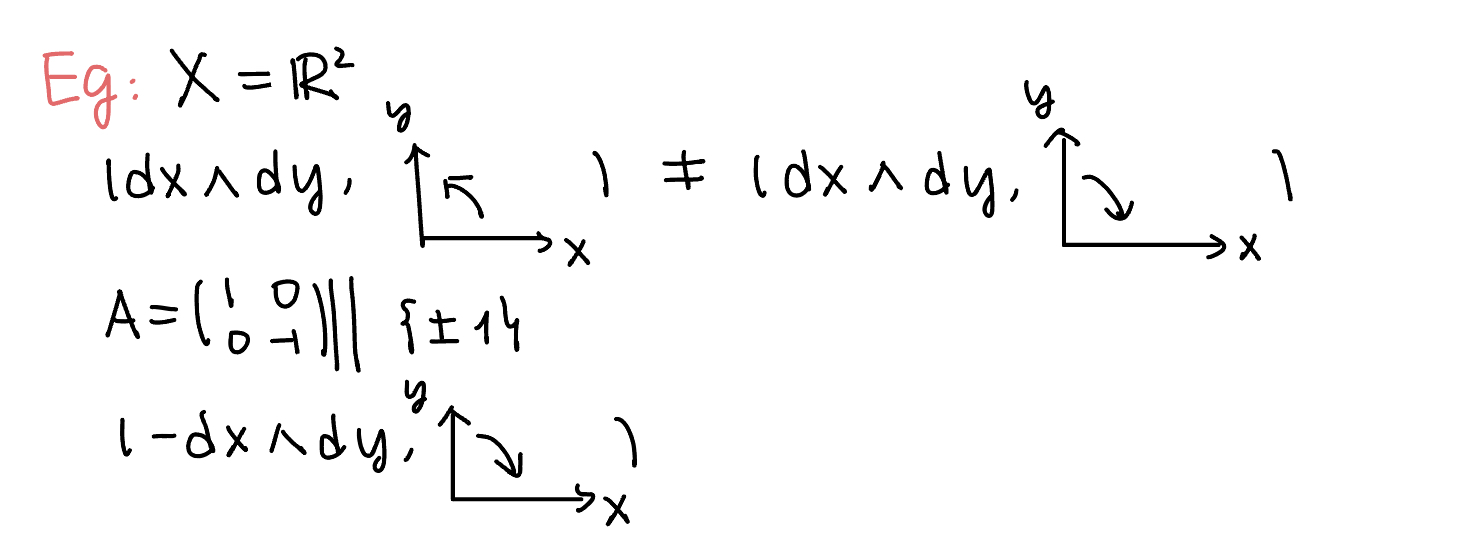
\includegraphics[width = 0.5\textwidth]{4.1.jpeg}
\end{center}

\subsubsection*{4.3: Volume forms on PL spaces}
Let $X$ be a PL space of dimension $n$ and $\mathcal{G}$ be a coefficient sheaf. The $G$-sheaf of volume forms with $\mathcal{G}$-coefficients is \[|\mathcal{G}^{n,0}_G| \coloneqq \mathcal{G}_G^{n,0} \times_{\{\pm 1\}}\mathrm{Or}_{X_G}.\] This is locally of rank $1$ over $\mathcal{G}_{X_G} / \mathcal{I}_n \mathcal{G}_{X_G}$. 

\begin{example}
    Let $X = \mathbf{R}^n$ with basis $x_1, \cdots, x_n$ and $\underline{\mathbf{R}}$ be the constant sheaf. Then $\omega_{\mathbf{R}^n} = d'x_1 \cdots d'x_n \in |\underline{\mathbf{R}}^{n,0}_{X_G}|$ is the canonical volume form.
\end{example}

One can naturally pullback such volume forms. If $f$ is a piecewise immersion of PL spaces, then one can also pushforward them by 4.1. 

\subsubsection*{4.4: Measures associated to vector volumes.}
We get a map of $G$-sheaves $|\mathcal{B}_{X_G}^{n,0}| \to \mathrm{Meas}_{\mathrm{Bor},X}$, where $\mathcal{B}$ stands for Borel coefficients. This is carried out in several steps. 

\begin{itemize}
    \item If $f \colon X \hookrightarrow \mathbf{R}^n$ is an embedding, where $X$ is a PL space, then we let $\lambda_{X,f}$ be the unique Borel measure on $X$ such that $f_* \lambda_{X,f}$ equals to the Lebesgue measure on $f(X)$. 
    \item For any $\omega \in |\mathcal{B}^{n,0}_{X_G}(Y)|$ where $Y$ is a PL subspace of $X$, let $\alpha^{\sharp}$ be a Borel function on a small neighborhood of $f(X)$ such that $f^*(\alpha^{\sharp} \omega_{\mathbf{R}^n}) = \omega.$ The Borel measure associated to $\omega$ is then \[\omega_{\mathrm{Bor}} \coloneqq f^*(|\alpha^{\sharp}|)\cdot \lambda_{X,f}.\] This measure is independent of the choice of $\alpha^{\sharp}$.
    \item Show that this construction respects inclusion of PL subspaces $Y' \subseteq Y$. 
    \item Glue to get a $G$-sheaf of Borel measures on $X$. 
\end{itemize}

If $\alpha^{\sharp} \in L^1_{\mathrm{loc}}$, then we can define a Radon measure $\omega_{\mathrm{Rad}}$ whose total variation equals $\omega_{\mathrm{Bor}}$. The construction of Borel measures commutes with pullback maps on cells. For piecewise immersions $f$, we have $(f_*\alpha)_{\mathrm{Bor}} \leq f_*(\alpha_{\mathrm{Bor}}).$


\subsubsection*{4.5: Calibration and integration of $(n,n)$-forms.}
The idea of integration an $(n,n)$-form on an $n$-dimensional PL space is to contract the $(0,n)$-part using a volume vector, and identify the $(n,0)$-part with the usual de Rham $n$-forms. Formally, we introduce the sheaf of calibrations on $X$, given by \[\mathrm{Cali}_X \coloneqq \mathcal{H}om_{X_G}(|\mathcal{G}^{n,0}_{X_G}|, \mathcal{G}_{X_G} / \mathcal{I}_n \mathcal{G}_{X_G}),\] which is $G$-locally of rank $1$ over $\mathcal{G}_{X_G} / \mathcal{I}_n \mathcal{G}_{X_G}$. For any PL cell $Y$ of dimension $n$, the following commutative diagram 

\begin{center}
\begin{tikzcd}
{\mathcal{G}^{0,n}_{X_G}(Y)} \arrow[r] \arrow[rd, "J"] & {|\mathcal{G}^{0,n}_{X_G}|(Y)} \arrow[r, "\mu"] \arrow[d, no head, Rightarrow] & \mathcal{G}_{X_G} / \mathcal{I}_n \mathcal{G}_{X_G}(Y) \arrow[d, "\simeq"]                  \\
                                                       & {\mathcal{G}^{n,0}_{X_G}(Y)}                                                   & \mathcal{G}_{X_G} / \mathcal{I}_n \mathcal{G}_{X_G} \times_{\{\pm 1\}} \mathrm{Or}_{X_G}(Y)
\end{tikzcd}
\end{center}
tensored with $\mathcal{G}^{n,0}_{X_G}$ gives us a map\footnote{This is because $\mathcal{G}^{n,0}_{X_G}$ has rank $1$ over $\mathcal{G}_{X_G} / \mathcal{I}_n \mathcal{G}_{X_G}$.} \[\mathcal{G}^{n,n}_{X_G} \to |\mathcal{G}^{n,0}_{X_G}|,\ \ \  \omega \mapsto \langle \omega, \mu\rangle.\] If $f \colon Y \to X$ is a piecewise immersion where $\dim(X), \dim(Y) \leq n$, then for any $(n,n)$-form $\omega$ on $X$ and any $\mu \in \mathrm{Cali}_Y$, we have a projection formula \[f_*\langle f^* \omega, \mu \rangle = \langle \omega, f_* \mu \rangle.\]

\subsubsection*{4.6: Calibration and integration of $(n-1,n)$-forms.}
Let $X$ be a PL space of dimension $n$ with a cell decomposition $\mathcal{C}$, and $\mu \in \Gamma(\mathrm{Cali}_X)$. Let $C \in \mathcal{C}$ be an $n$-dimensional cell, with $F < C$ be an $(n-1)$-dimensional cell. For any $(n-1,n)$-form $\omega$, we can define an $(n-1,n)$-form on $F$ with respect to the structure $F < C$, denoted $\langle \omega, \mu \rangle |_{(F,C)}$. Further, there exists a unique $n-1$-form $\langle \omega, \mu\rangle_{\mathcal{C}}$ on the union of all $(n-1)$-cells of $\mathcal{C}$ such that for any $(n-1)$-cell $F$, the following is satisfied: 
\[\langle \omega, \mu \rangle_{\mathcal{C}} |_F = \sum_{C \supseteq F, C \in \mathcal{C}_n} \langle \omega, \mu \rangle|_{\langle F, C \rangle}.\]
Here $\mathcal{C}_n \subseteq \mathcal{C}$ is the collection of all $n$-dimensional cells. It turns out that this form is actually independent of the choice of the decomposition $\mathcal{C}$, and therefore is simply denoted as $\langle \omega, \mu \rangle$, an $(n-1)$-form on $X$. This construction again satisfies a version of the projection formula, and moreover given any locally finite $G$-covering of $X$, there is an inclusion-exclusion formula for the calculation of this form. 

We define integrations
\begin{align*}
    \int_X \langle d'\omega, \mu \rangle &\coloneqq \sum_{C \in \mathcal{C}_n} \int_C \langle d' \omega, \mu\rangle,\\
    \int_{\partial X} \langle \omega, \mu \rangle &\coloneqq \sum_{D \in \mathcal{C}_{n-1}} \sum_{D\subseteq C \in \mathcal{C}_n} \int_D \langle \omega, \mu \rangle.
\end{align*}

\begin{theorem}[Stokes' formula]
    Let $\omega$ be an $(n-1,n)$-form with $C^1_c$-coefficient on $X$. Then \[\int_X \langle d'\omega, \mu \rangle = \int_{\partial X} \langle \omega, \mu \rangle.\]
\end{theorem}

\begin{theorem}[Green's formula]
    Let $\alpha, \beta$ be symmetric $(p,p), (q,q)$-forms on $X$ with $p+q = n-1$. Suppose either a) their coefficients are $C^2_c$, or b) $\mathrm{supp}(\alpha) \cap \mathrm{supp}(\beta)$ is compact, then 
    \[\int_X \langle \alpha \wedge d'd''\beta - d'd''\alpha \wedge \beta, \mu \rangle = \int_{\partial X} \langle \alpha \wedge d'' \beta - d'' \alpha \wedge \beta, \mu \rangle. \]
\end{theorem}

\subsection*{Chapter 5: Calibrated $G$-tropical spaces}

\subsubsection*{5.1: Chorded $G$-tropical spaces.} Given a $G$-tropical space $X$, the intersection of two closed PL subspaces is not necessarily PL. To avoid this issue, we need to single out a paricular collection $\mathcal{S}$ of PL subspaces of $X$ and of any $V \in \mathrm{Dom}(X)$ that are stable under finite unions and intersections. Elements in $\mathcal{S}$ are called elementarily skeletal subsets, and $(X, \mathcal{S})$ is a chorded $G$-tropical space. Subsets of $X$ that are $G$-locally elementarily skeletal are call skeletal. For any point $x \in X$ that lie in some skeletal subset, we say $x$ is skeletal. If $X$ is a PL space, then one can simply take all PL subspaces are skeletal subsets. 

Since by definition, the elementarily skeletal subsets (ESS) are PL subspaces, we can talk about their calibrations by Chapter 4. Definition 5.1.6 gives the notion of calibrated skeletal subsets purely of dimension $p$. Such subsets form a lattice. 

\subsubsection*{5.2: Vertebrate $G$-tropical spaces.} Let $X$ be a $G$-tropical space with $d_{\mathrm{trop}} \leq n$, and let $f \colon V \to \mathbf{R}^n$ be a $G$-tropical chart of $X$. The subset $\Sigma_f^{(n)}$ is the collection of all $x \in V$ with $d_{\mathrm{trop},x}(f) = n$. This is closed (possibly empty) in $X$. If $X$ is chorded and all such $\Sigma_f^{(n)}$ are skeletal, then $X$ is called a vertebrate $G$-tropical space. For example, PL spaces are vertebrate. A consequence is that, in a vertebrate $G$-tropical space, PL subspaces of pure dimensions are skeletal (see Proposition 5.2.6). The notion of (very) richness measures the amplitude of compact skeletal subsets of $X$. Later, the book will equip any separeted, pure-dimensional $k$-analytic spaces over any complete field non-archimedean field $k$ a vertebrate $G$-tropical structure, but the essential ingredients are already listed in Example 5.2.8. 

\subsubsection*{5.3: Strong support.} Let $X$ be a vertebrate $G$-tropical space of dimension $n$. Let $\omega$ be a $G$-form of type $(p,q)$ on $X$ where $\max(p,q) = n$. A closed skeletal subset $\Sigma$ of $X$ strongly supports $\omega$ if for any other closed skeletal subset $T$ containing $\Sigma$, the form $\omega|_T$ is $\omega|_{\Sigma}$ extend by zero. Strong support is $G$-local. If $\Sigma$ strongly supports $\omega$, then so does $\Sigma^{(n)}$. If $\omega$ is tropicalized by a $G$-tropical chart $f$, then $\Sigma_f^{(n)}$ already strongly supports $\omega$. In general, if $X$ is paracompact or $\omega$ is compactly supported, then there always exists some closed skeletal subset of $X$ that strongly supports $\omega$. If $\Sigma$ strongly supports $\omega$, then the support (see 3.2) of $\omega|_{\Sigma}$ equals to the support of $\omega$ on $X$. 

\subsubsection*{5.4: Agreeable charts, tropical polyhedrons and cones.} Let $X$ be a vertebrate $G$-tropical space of dimension $n$, and $f \colon V \to E$ be a $G$-tropical chart. A subset $C \subseteq X$ is an $f$-cell if it is an $f$-cell of the PL subspace $\Sigma_f^{(n)}$. For example, if $f$ is homeomorphism onto its image, then the inverse images of $n$-dimensional cells in $f(V)$ are $f$-cells. Such $f$ is called agreeable if $f(\Sigma_f^{(n)})$ is PL in $E$ anad $f|_{\Sigma_f^{(n)}}$ is proper onto its image. It this is the case, let $\Pi_f$ denote the PL space $f(\Sigma_f^{(n)})$ and is called the tropical polyhedron of $f$. 

Let $\mathcal{C}$ (resp. $\mathcal{C}'$, but possibly in a subset of $\Sigma_f^{(n)}$) be a cellular decomposition of $\Sigma_f^{(n)}$. Pick a point $x \in \Sigma_f^{(n)}$, and let $V$ (resp. $V')$ be the union of $n$-cells in $\mathcal{C}$ (resp. $\mathcal{C}'$) that contains $x$. By topological properties, the germs of the polyhedra $f(V)$ and $f(V')$ at $f(x)$ agree, which is a cone with vertex $f(x)$, is called a tropical cone at $f(x)$ and denoted by $\Pi_{f,x}$. 

%This is a compact PL neighborhood of $x$. Moreover, $f|_V$ is a piecewise immersion of $V$ that maps each $C$ in the union to a strong cell in $E$. Pick any other open paracompact $W'$ that is a neighborhood of $x$, and let $\mathcal{C}'$ be a cellular decomposition of $\Sigma_f^{(n)} \cap W'$. Moreover, let $V'$ be the union of $n$-cells in $\mathcal{C}'$ that contains $x$. Then $V \cap V'$ is a compact PL neighborhood of $x$ in $V$. By topology, there exists a compact PL neighborhood $U$ of $f(x)$ with $f^{-1}(U) \subseteq V \cap V'$. That is to say, the polyhedra $f(V)$ and $f(V')$ agree in a neighborhood of $f(x)$.  

\subsubsection*{5.5: Calibrated $G$-tropical spaces.}
Let $X$ be a vertebrate $G$-tropical space of dimension $n$. It is calibrated if every skeletal subset $\Sigma$ of $X$ is equipped with a strictly positive vector volume $\mu_\Sigma$ that is stable under taking skeletal subsets. This recovers the calibration of PL spaces. The tropical cone $\Pi_{f,x}$ is canonically calibrated. 

\subsubsection*{5.6: Volume forms on vertebrate $G$-tropical spaces.} Let $p \leq n$ be integers, and $X$ is a calibrated $G$-tropical space. We say it is of level $n$ if $\dim{X} \leq n$. This section defines $p$-vector volumes on $X$. 

\subsubsection*{5.7: Measures associated to $p$-dimensional volume forms.}

\subsubsection*{5.8: Integration of differential forms.}

\subsubsection*{5.9: Boundary measure.}

\subsubsection*{5.10: Integrals and tropicalizations.}

\subsubsection*{5.11: Stokes' and Green's formulae.}

\subsection*{Chapter 7: Currents on $G$-tropical spaces}

\subsubsection*{}


\bibliographystyle{alpha}
\bibliography{references}

\end{document}